\subsection{Arquitetura ETL/DSA}
A arquitetura implementada para o sistema de suporte analítico fundamenta-se num processo de integração que reúne dados provenientes de fontes heterogéneas, aplica as transformações necessárias e prepara a sua posterior carga no repositório analítico. Esta secção apresenta uma visão geral do fluxo de dados e dos componentes envolvidos, permitindo compreender a organização da informação antes da sua disponibilização no \textit{Data Warehouse}.

A Figura \ref{fig:arquiteturaetl} ilustra a arquitetura do processo ETL desenhado para o sistema. À esquerda da figura, identificam-se as fontes de dados, que incluem os ficheiros disponibilizados pelo ICNF, dados meteorológicos em formato bruto e informação externa, como a cobertura mediática.
O fluxo de dados prossegue para a área de preparação (\textit{Staging Area}), onde ocorre o processamento central. Esta camada engloba estruturas de suporte, um espaço de quarentena para validação de qualidade e a lógica de transformação que organiza os dados em zonas específicas.
Por fim, após a devida preparação e limpeza, a informação é encaminhada para a área de carregamento, sendo persistentemente armazenada no \textit{Data Warehouse}.

\begin{figure}[htbp]
	\centering
	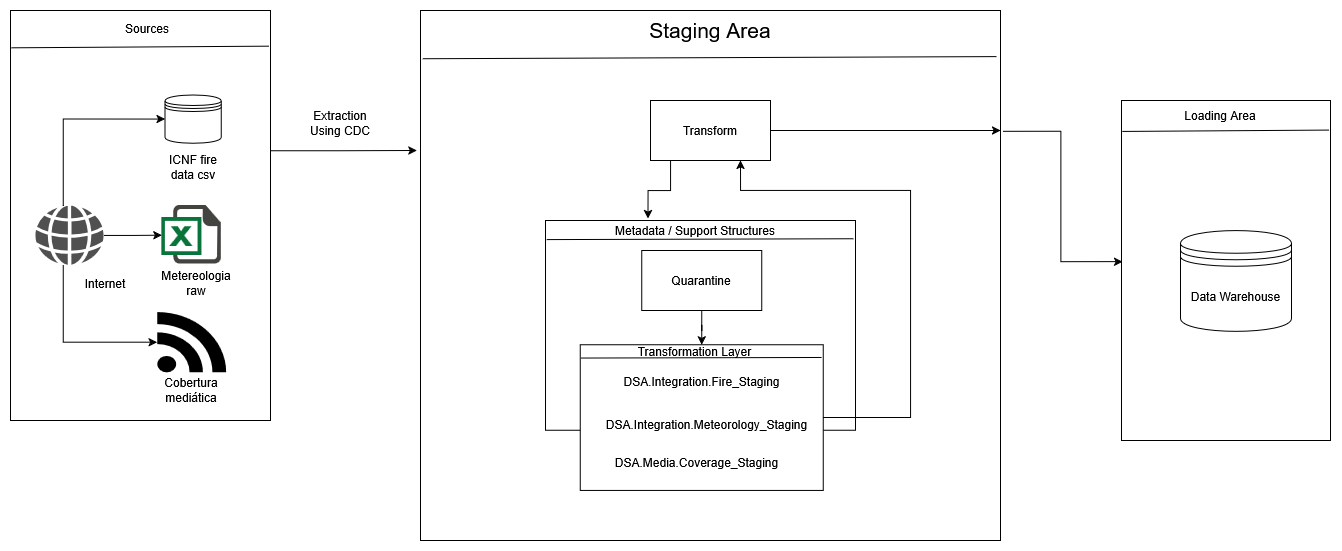
\includegraphics[width=1.0\linewidth]{imagens/Arquitetura_ETL}
	\caption{Arquitetura ETL (Estrutura da DSA)}
	\label{fig:arquiteturaetl}
\end{figure}